\section{M21}\label{sec:m21}

 Listamos, na tabela \ref{tab:comandos}, algumas opções úteis do comando \verb|./m21|. Foram usadas para a elaboração de materiais pré-composicionais, apresentados na seção \ref{sec:resultados}. 

Um manual de instalação e operação mais detalhado está disponível junto com o código-fonte\footnote{Disponível em \url{https://www.github.com/jahpd/m21/doc/manual.pdf}.}.

\begin{table}
\caption{Tabela das opções utilizadas para produção e análise de um arquivo partiturável. \textbf{Fonte}: autor.}
\small
    \begin{tabular}{| p{3cm} | p{3cm} | p{2.25cm} | p{5.75cm} |}
    \hline 
    \hline 

    \textbf{Nome} & 
    \textbf{Comando} &
    \textbf{Abreviação} &
    \textbf{Execução}\\

    \hline

    \textbf{Compositor} 
    & \verb|--composer|
    & \verb|-c|             
    & Campo de procura no corpus pelo nome de um compositor. Usado em conjunto com a opção ``Index''. \\
    \hline

    \textbf{Index} 
    & \verb|--index|    
    & \verb|-i|             
    & Indexação de uma peça (catálogo, p.e., bwv123). Usado em conjunto com a opção ``Compositor'' \\
    \hline

    \textbf{Composição Assistida por Computador} 
    & \verb|--CAC|  
    & \verb|-C|             
    & \emph{Flag} indicativa de uma operação de transformação em uma partitura. Usada em conjunto, as opções ``Compositor'' e ``Index''.\\
    \hline

     \textbf{Glitch} 
    & \verb|--glitch|      
    & \verb|-g|              
    & \emph{Flag} indicativa do tipo de operação de transformação. A peça é desorganizada e verticalizada em blocos harmônicos, de maneira randômica, limitada apenas por regras de tessitura do piano. \\
    \hline

    \textbf{Apresentar em um editor de partituras} 
    & \verb|--Show|       
    & \verb|-S|             
    & \emph{Flag} indicativa que, o resultado obtido será executado em um editor de partituras apropriado, no caso deste trabalho, o \cite{musescore_2015}.\\
    \hline
    
    \textbf{Plotar gráficos analíticos} 
    & \verb|--plot-*|       
    & -                                          
    & \emph{Flag} indicativa que um gráfico analítico será gerado. O Símbolo ``*'' representa a diversidade dos tipos de gráficos possíveis. \\
    \hline
    \hline
   
    \end{tabular}
\label{tab:comandos}
\end{table}
 
\subsection{Análise orientada por gráficos}

Histogramas e outros gráficos podem ser gerados para de diferentes aspectos de uma música.  Por exemplo, na figura \ref{fig:pitch-space-bwv1-histogram}, apresentamos um histograma do espaço de alturas (\emph{pitch-space}) do sexto movimento do BWV1 de J.S.Bach. O gráfico foi gerado com o auxílio  do comando apresentado no código \ref{code:plot}

\begin{figure}
\begin{minted}[linenos,frame=leftline,fontsize=\scriptsize]{python}
./m21 --show --composer bach --index bwv1 --plot-histogram-pitch-space
\end{minted}
\label{code:plot}
\end{figure}

\begin{figure}[h]
  \centering
  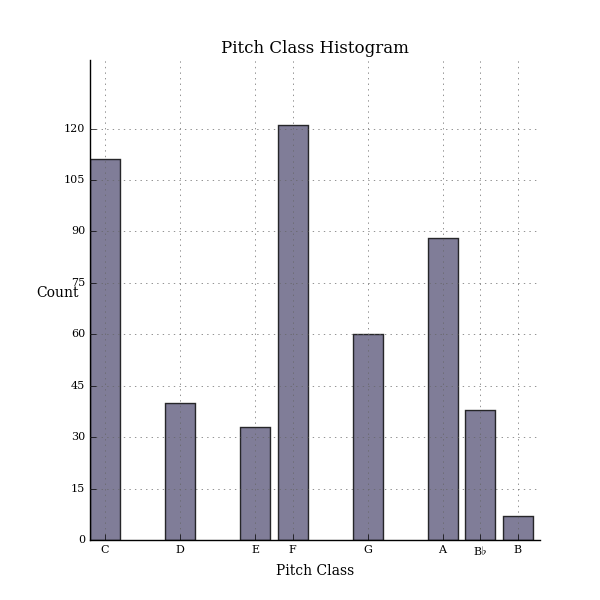
\includegraphics[scale=0.71]{../analysis/bwv1/pitch-class.png}
  \caption{Histograma de \emph{pitch-class} do BWV1.6, utilizando o comando \textbf{Fonte}: autor.}
    \label{fig:pitch-space-bwv1-histogram}
\end{figure}

%  \verb|./m21 --show --composer bach --index bwv1 --plot-histogram-pitch-space|. \textbf{Fonte}: autor.}
